\documentclass{article}

\usepackage{fancyhdr}
\usepackage{extramarks}
\usepackage{amsmath}
\usepackage{amsthm}
\usepackage{amsfonts}
\usepackage{tikz}
\usepackage[plain]{algorithm}
\usepackage{algpseudocode}
\usepackage{xcolor}
\usepackage{enumerate}
\usepackage{amssymb}
\usepackage{graphicx}
\usepackage{float} 
\usepackage{subfigure}


\usetikzlibrary{automata,positioning}

\topmargin=-0.45in
\evensidemargin=0in
\oddsidemargin=0in
\textwidth=6.5in
\textheight=9.0in
\headsep=0.25in

\linespread{1.1}

\pagestyle{fancy}
\lhead{\hmwkAuthorName}
\chead{\hmwkClass\ (\hmwkClassInstructor\ \hmwkClassTime): \hmwkTitle}
\rhead{\firstxmark}
\lfoot{\lastxmark}
\cfoot{\thepage}

\renewcommand\headrulewidth{0.4pt}
\renewcommand\footrulewidth{0.4pt}

\setlength\parindent{0pt}

\newcommand{\enterProblemHeader}[1]{
    \nobreak\extramarks{}{Problem \arabic{#1} continued on next page\ldots}\nobreak{}
    \nobreak\extramarks{Problem \arabic{#1} (continued)}{Problem \arabic{#1} continued on next page\ldots}\nobreak{}
}

\newcommand{\exitProblemHeader}[1]{
    \nobreak\extramarks{Problem \arabic{#1} (continued)}{Problem \arabic{#1} continued on next page\ldots}\nobreak{}
    \stepcounter{#1}
    \nobreak\extramarks{Problem \arabic{#1}}{}\nobreak{}
}

\setcounter{secnumdepth}{0}
\newcounter{partCounter}
\newcounter{homeworkProblemCounter}
\setcounter{homeworkProblemCounter}{1}
\nobreak\extramarks{Problem \arabic{homeworkProblemCounter}}{}\nobreak{}

\newenvironment{homeworkProblem}[1][-1]{
    \ifnum#1>0
        \setcounter{homeworkProblemCounter}{#1}
    \fi
    \section{Problem \arabic{homeworkProblemCounter}}
    \setcounter{partCounter}{1}
    \enterProblemHeader{homeworkProblemCounter}
}{
    \exitProblemHeader{homeworkProblemCounter}
}

\newcommand{\hmwkTitle}{HW\ \#1}
\newcommand{\hmwkDueDate}{July 14, 2023}
\newcommand{\hmwkClass}{Tandon CS Bridge}
\newcommand{\hmwkClassTime}{Extended 24-week}
\newcommand{\hmwkClassInstructor}{Ratan Dey}
\newcommand{\hmwkAuthorName}{\textbf{Kunhua Huang}}
\newcommand{\hmwkNYUID}{kh4092}

\title{
    \vspace{2in}
    \textmd{\textbf{\hmwkClass:\ \hmwkTitle}}\\
    \normalsize\vspace{0.1in}\small{Due\ on\ \hmwkDueDate}\\
    \vspace{0.1in}\large{\textit{\hmwkClassInstructor\, \hmwkClassTime}}
    \vspace{3in}
}

\author{
    \vspace{0.1in}
    \textmd{\hmwkAuthorName}\\
    \text{\hmwkNYUID}
}
\date{}

\renewcommand{\part}[1]{\textbf{\large Part \Alph{partCounter}}\stepcounter{partCounter}\\}

%
% Various Helper Commands
%

% Useful for algorithms
\newcommand{\alg}[1]{\textsc{\bfseries \footnotesize #1}}

% For derivatives
\newcommand{\deriv}[1]{\frac{\mathrm{d}}{\mathrm{d}x} (#1)}

% For partial derivatives
\newcommand{\pderiv}[2]{\frac{\partial}{\partial #1} (#2)}

% Integral dx
\newcommand{\dx}{\mathrm{d}x}

% Alias for the Solution section header
\newcommand{\solution}{\textbf{\large Solution}}

\newcommand\logeq{\mathrel{\raisebox{.66pt}{:}}\Leftrightarrow}

% Probability commands: Expectation, Variance, Covariance, Bias
\newcommand{\E}{\mathrm{E}}
\newcommand{\Var}{\mathrm{Var}}
\newcommand{\Cov}{\mathrm{Cov}}
\newcommand{\Bias}{\mathrm{Bias}}

\begin{document}

\maketitle

\pagebreak

\begin{homeworkProblem}
    A. Convert the following numbers to	their decimal representation. Show your work.
    
    \begin{enumerate}
        \item $10011011_2$ =
        \item $456_7$ =
        \item $38A_{16}$ =
        \item $2214_5$ =
    \end{enumerate}

    \textbf{Solution}
    \begin{center}
        \begin{enumerate}
            \item $10011011_2=1*2^7+0*2^6+0*2^5+1*2^4+1*2^3+0*2^2+1*2^1+1*2^0=\boxed{154}$
            \item $456_7=4*7^2+5*7^1+6*7^0=\boxed{237}$
            \item $38A_{16}=3*16^2+8*16^1+A*16^0=\boxed{906}$
            \item $2214_5=2*5^3+2*5^2+1*5^1+4*5^0=\boxed{309}$
        \end{enumerate}
    \end{center}
    
    B. Convert the following numbers to their binary representation:

    \begin{enumerate}
        \item $69_{10}$ =
        \item $485_{10}$ =
        \item $6D1A_{16}$ =
    \end{enumerate}

    \textbf{Solution}
        \begin{enumerate}
            \item Step 1:\\
                \begin{center}
                    $69\equiv1\pmod2$\\
                    $34\equiv0\pmod2$\\
                    $17\equiv1\pmod2$\\
                    $8\equiv0\pmod2$\\
                    $4\equiv0\pmod2$\\
                    $2\equiv0\pmod2$\\
                \end{center}

                Step 2:\\
                Add a leading 1 and concatenate the remainders unwards:\\
                The result is \boxed{$1000101$}.
            \item Step 1:\\
            \begin{center}
                $485\equiv1\pmod2$\\
                $242\equiv0\pmod2$\\
                $121\equiv1\pmod2$\\
                $60\equiv0\pmod2$\\
                $30\equiv0\pmod2$\\
                $15\equiv1\pmod2$\\
                $7\equiv1\pmod2$\\
                $3\equiv1\pmod2$\\
            \end{center}

                Step 2:\\
                Add a leading 1 and concatenate the remainders unwards:\\
                The result is \boxed{$111100101$}.
            \item 
                The binary values of 6, D, 1, A are 0110, 1101, 0001, 1010, respectively.\\
                Thus, the binary value of 6D1A is \boxed{$0110110100011010$}.
        \end{enumerate}
    
    C. Convert the following numbers to their hexadecimal representation:
   
    \begin{enumerate}
        \item $1101011_2$ =
        \item $895_{10}$ =
    \end{enumerate}
    
    \textbf{Solution}
        \begin{enumerate}
            \item
                Add a leading 0 to make it 8-bit: 0110 1011\\
                The hexadecimal values of 0110, 1011 are 6, B, respectively.\\
                Thus, the hexadecimal value of 0110 1011 is 6B.
            \item Step 1:\\
            \begin{center}
                $895\equiv15(F)\pmod{16}$\\
                $55\equiv7\pmod{16}$\\
                $48=3*16$\\
            \end{center}

                Step 2:
                The hexadecimal value is \boxed{$37F$}.
        \end{enumerate}
\end{homeworkProblem}

\pagebreak

\begin{homeworkProblem}
    Solve the following, do all calculation in the given base. Show your work.
    \begin{enumerate}
        \item $7566_8+4515_8=$
        \item $10110011_2+1101_2=$
        \item $7A66_{16}+45C5_{16}=$
        \item $3022_5+2433_5=$
    \end{enumerate}


    
    \textbf{Solution}
    \begin{enumerate}
        \item
        \begin{center}
            \begin{tabular}{lr}
                &$7_{\textcolor{white}{a}}5_{\textcolor{white}{a}}6_{\textcolor{white}{a}}6_{\textcolor{white}{a}}$\\
                +&$4_15_11_15_{\textcolor{white}{a}}$\\
                \hline
                &$1_{\textcolor{white}{a}}4_{\textcolor{white}{a}}3_{\textcolor{white}{a}}0_{\textcolor{white}{a}}3_{\textcolor{white}{a}}$\\
            \end{tabular}
        \end{center}
        The result is \boxed{14303_{(8)}}.
        \item
        \begin{center}
            \begin{tabular}{lr}
                &$1_{\textcolor{white}{a}}0_{\textcolor{white}{a}}1_{\textcolor{white}{a}}1_{\textcolor{white}{a}}0_{\textcolor{white}{a}}0_{\textcolor{white}{a}}1_{\textcolor{white}{a}}1_{\textcolor{white}{a}}$\\
                +&$0_{\textcolor{white}{a}}0_10_10_11_11_10_11_{\textcolor{white}{a}}$\\
                \hline
                &$1_{\textcolor{white}{a}}1_{\textcolor{white}{a}}0_{\textcolor{white}{a}}0_{\textcolor{white}{a}}0_{\textcolor{white}{a}}0_{\textcolor{white}{a}}0_{\textcolor{white}{a}}0_{\textcolor{white}{a}}$\\
            \end{tabular}
        \end{center}
        The result is \boxed{11000000_{(2)}}.
        \item 
        \begin{center}
            \begin{tabular}{lr}
                &$7_{\textcolor{white}{a}}A_{\textcolor{white}{a}}6_{\textcolor{white}{a}}6_{\textcolor{white}{a}}$\\
                +&$4_15_1C_{\textcolor{white}{a}}5_{\textcolor{white}{a}}$\\
                \hline
                &$C_{\textcolor{white}{a}}0_{\textcolor{white}{a}}2_{\textcolor{white}{a}}B_{\textcolor{white}{a}}$\\
            \end{tabular}
        \end{center}
        The result is \boxed{C02B_{(16)}}.
        \item
        \begin{center}
            \begin{tabular}{lr}
                &$3_{\textcolor{white}{a}}0_{\textcolor{white}{a}}2_{\textcolor{white}{a}}2_{\textcolor{white}{a}}$\\
                +&$2_14_13_13_{\textcolor{white}{a}}$\\
                \hline
                &$1_{\textcolor{white}{a}}1_{\textcolor{white}{a}}0_{\textcolor{white}{a}}1_{\textcolor{white}{a}}0_{\textcolor{white}{a}}$\\
            \end{tabular}
        \end{center}
        The result is \boxed{11010_{(5)}}.
    \end{enumerate}    
\end{homeworkProblem}

\pagebreak

\begin{homeworkProblem}
    A. Convert the following numbers to their 8-bits two's complement representation. Show your work.
    \begin{enumerate}
        \item $124_{10}=$
        \item $-124_{10}=$
        \item $109_{10}=$
        \item $-79_{10}=$
    \end{enumerate}

    \textbf{Solution}
    \begin{enumerate}
        \item Get the binary value of 124 and add a leading 0, we have \boxed{01111100_{8 bit 2's comp}}
        \item Step 1: Get the binary value of 124 and add a leading 0, which is 01111100\\
        Step 2: Get its complement 10000011\\
        Step 3:\\
        \begin{center}
            \begin{tabular}{lr}
                &$10000011$\\
                +&$1$\\
                \hline
                &$10000100$\\
            \end{tabular}
        \end{center}
        The result is \boxed{10000100_{8 bit 2's comp}}.
        \item Get the binary value of 109 and add a leading 0, we have \boxed{01101101_{8 bit 2's comp}}
        \item Step 1: Get the binary value of 79 and add a leading 0, we have 01001111\\
        Step 2: Get its complement 10110000\\
        Step 3:\\
        \begin{center}
            \begin{tabular}{lr}
                &$10110000$\\
                +&$1$\\
                \hline
                &$10110001$\\
            \end{tabular}
        \end{center}
        The result is \boxed{10110001_{8 bit 2's comp}}.
    \end{enumerate}
\end{homeworkProblem}

\pagebreak

\begin{homeworkProblem}
    Solve the following questions from the Discrete Math zyBook:
    \begin{enumerate}
        \item Exercise 1.2.4, sections b, c\\
        \\
        Write a truth table for each expression.
        \begin{enumerate}
            \item \[\neg (p \lor q)\]
            \item \[r \lor (p \land \neg q)\]
        \end{enumerate}

        \textbf{Solution}
        \begin{enumerate}[(a)]
            \item \begin{center}
                \begin{tabular}{||c | c | c | c ||} 
                 \hline
                 $p$ & $q$ & $p \lor q$ & $\neg (p \lor q)$ \\ [0.5ex] 
                 \hline\hline
                 T & T & T & F \\ 
                 \hline
                 T & F & T & F \\
                 \hline
                 F & T & T & F \\
                 \hline
                 F & F & F & T \\ [1ex] 
                 \hline
                \end{tabular}
                \end{center}
            \vspace{0.1in}
            \item \begin{center}
                \begin{tabular}{||c | c | c | c | c | c ||} 
                    \hline
                    $r$ & $p$ & $q$ & $\neg q$ & $p \land \neg q$ & $r \lor (p \land \neg q)$ \\ [0.5ex] 
                    \hline\hline
                    T & T & T & F & F & T\\ 
                    \hline
                    T & T & F & T & T & T\\
                    \hline
                    T & F & T & F & F & T\\
                    \hline
                    T & F & F & T & F & T\\
                    \hline
                    F & T & T & F & F & F\\
                    \hline
                    F & T & F & T & T & T\\
                    \hline
                    F & F & T & F & F & F\\
                    \hline
                    F & F & F & T & F & F\\ [1ex] 
                    \hline
                \end{tabular}
                \end{center}
                \vspace{0.2in}
        \end{enumerate}
        \item Exercise 1.3.4, sections b, d\\
        \\
        Give a truth table for each expression.
        \begin{enumerate}
            \item \[(p \rightarrow q) \rightarrow (q \rightarrow p)\]
            \item \[(p \leftrightarrow q) \oplus (p \leftrightarrow \neg q) \]
        \end{enumerate}

        \textbf{Solution}
        \begin{enumerate}[(a)]
            \item \begin{center}
                \begin{tabular}{||c | c | c | c | c ||} 
                 \hline
                 $p$ & $q$ & $(p \rightarrow q)$ & $(q \rightarrow p)$ & $(p \rightarrow q) \rightarrow (q \rightarrow p)$ \\ [0.5ex] 
                 \hline\hline
                 T & T & T & T & T \\ 
                 \hline
                 T & F & F & T & T\\
                 \hline
                 F & T & T & F & F\\
                 \hline
                 F & F & T & T & T\\ [1ex] 
                 \hline
                \end{tabular}
                \end{center}
            \vspace{0.1in}
            \item \begin{center}
                \begin{tabular}{||c | c | c | c | c | c ||} 
                    \hline
                    $p$ & $q$ & $\neg q$ & $(p \leftrightarrow q)$ & $(p \leftrightarrow \neg p)$ & $(p \leftrightarrow q) \oplus (p \leftrightarrow \neg q)$ \\ [0.5ex] 
                    \hline\hline
                    T & T & F & F & T & T\\ 
                    \hline
                    T & F & T & T & T & F\\
                    \hline
                    F & T & F & T & F & T\\
                    \hline
                    F & F & T & T & T & F\\ [1ex] 
                    \hline
                   \end{tabular}
                \end{center}
                \vspace{0.2in}
        \end{enumerate}
    \end{enumerate}
\end{homeworkProblem}

\pagebreak

\begin{homeworkProblem}
    Solve the following questions from the Discrete Math zyBook:
    \begin{enumerate}
        \item Exercise 1.2.7, sections b, c\\
        \\
        Consider the following pieces of identification a person might have in order to apply for a credit card:\\
        \\
        B: Applicant presents a birth certificate.\\
        D: Applicant presents a driver's license.\\
        M: Applicant presents a marriage license.\\
        \\
        Write a logical expression for the requirements under the following conditions:
        \begin{enumerate}
            \item The applicant must present at least two of the following forms of identification: birth certificate, driver's license, marriage license.
            \item Applicant must present either a birth certificate or both a driver's license and a marriage license.
        \end{enumerate}
        
        \textbf{Solution}
        \begin{enumerate}
            \item 
                \[[B \land (D \lor M)] \lor [(B \lor D) \land M] \lor [(B \lor M) \land D]\]
            \item   
                \[B \lor (D \land M)\]
        \end{enumerate}
        \item Exercise 1.3.7, sections b - e\\
        \\
        Define the following propositions:\\
        \\
        s: a person is a senior\\
        y: a person is at least 17 years of age\\
        p: a person is allowed to park in the school parking lot\\
        \\
        Express each of the following English sentences with a logical expression:
        \begin{enumerate}
            \item A person can park in the school parking lot if they are a senior or at least seventeen years of age.
            \item Being 17 years of age is a necessary condition for being able to park in the school parking lot.
            \item A person can park in the school parking lot if and only if the person is a senior and at least 17 years of age.
            \item Being able to park in the school parking lot implies that the person is either a senior or at least 17 years old.
        \end{enumerate}

        \textbf{Solution}
        \begin{enumerate}
            \item \[(s \lor y) \rightarrow p\]
            \item \[y \rightarrow p\]
            \item \[p \rightarrow (s \land y)\]
            \item \[p \rightarrow (s \lor y)\]
        \end{enumerate}
        \item Exercise 1.3.9, sections c, d\\
        \\
        Use the definitions of the variables below to translate each English statement into an equivalent logical expression.\\
        \\
        y: the applicant is at least eighteen years old\\
        p: the applicant has parental permission\\
        c: the applicant can enroll in the course\\
        \\
        \begin{enumerate}
            \item The applicant can enroll in the course only if the applicant has parental permission.
            \item Having parental permission is a necessary condition for enrolling in the course.
        \end{enumerate}

        \textbf{Solution}
        \begin{enumerate}
            \item \[c \rightarrow p\]
            \item \[c \rightarrow p\]
        \end{enumerate}
    \end{enumerate}
\end{homeworkProblem}

\pagebreak

\begin{homeworkProblem}
    Solve the following questions from the Discrete Math zyBook:
    \begin{enumerate}
        \item Exercise 1.3.6, sections b - d\\
        \\
        Give an English sentence in the form "If...then..." that is equivalent to each sentence.\\
        \\
        \begin{enumerate}
            \item Maintaining a B average is necessary for Joe to be eligible for the honors program.
            \item Rajiv can go on the roller coaster only if he is at least four feet tall.
            \item Rajiv can go on the roller coaster if he is at least four feet tall.
        \end{enumerate}

        \textbf{Solution}
        \begin{enumerate}
            \item If Joe is eligible for the honors program, then he is maintaning a B average.
            \item If Rajiv is not at least four feet tall, then he cannot go on the roller coaster.
            \item If Rajiv is at least four feet tall, then he can go on the roller coaster.
        \end{enumerate}
        
        \item Exercise 1.3.10, sections c - f\\
        \\
        The variable p is true, q is false, and the truth value for variable r is unknown. Indicate whether the truth value of each logical expression is true, false, or unknown.\\
        \\
        \begin{enumerate}
            \item \[(p \lor r) \leftrightarrow (q \land r)\]
            \item \[(p \land r) \leftrightarrow (q \land r)\]
            \item \[p \rightarrow (r \lor q)\]
            \item \[(p \land q) \rightarrow r\]
        \end{enumerate}

        \textbf{Solution}
        \begin{enumerate}
            \item false
            \item false
            \item unknown
            \item true
        \end{enumerate}
    \end{enumerate}
\end{homeworkProblem}

\pagebreak

\begin{homeworkProblem}
    Solve Exercise 1.4.5, sections b - d, from the Discrete Math zyBook\\
    \\
    Define the following propositions:\\
    \\
    j: Sally got the job.\\
    l: Sally was late for her interview\\
    r: Sally updated her resume.\\
    \\
    Express each pair of sentences using logical expressions. Then prove whether the two expressions are logically equivalent.\\
    \begin{enumerate}
        \item If Sally did not get the job, then she was late for her interview or did not update her resume.\\
        If Sally updated her resume and was not late for her interview, then she got the job.
        \item If Sally got the job then she was not late for her interview.\\
        If Sally did not get the job, then she was late for her interview.
        \item If Sally updated her resume or she was not late for her interview, then she got the job.\\
        If Sally got the job, then she updated her resume and was not late for her interview.
    \end{enumerate}

    \textbf{Solution}
    \begin{enumerate}
        \item Sentence 1: \[\neg j \rightarrow (l \lor \neg r)\]
        \[\iff j \lor (l \lor \neg r)\] (Conditional Identities)\\
        \\
        Sentence 2: \[(r \land \neg l) \rightarrow j\]
        \[\iff \neg (r \land \neg l) \lor j\] (Conditional Identities)
        \[\iff (\neg r \lor l) \lor j\] (De Morgan's Laws)
        \[\iff j \lor (l \lor \neg r)\] (Commutative Laws)\\
        \\
        \[\therefore Sentence\;1 \equiv Sentence\;2\]\\
        \item Sentence 1: \[j \rightarrow \neg l\]\\
        Sentence 2: \[\neg j \rightarrow l\]
        \\
        \[\therefore Sentence\;1 \not\equiv Sentence\;2\]\\
        \\
        \item Sentence 1: \[(r \lor \neg l) \rightarrow j\]
        \\
        Sentence 2: \[j \rightarrow (r \land \neg l)\]
        \\
        Truth Table: \begin{center}
            \begin{tabular}{||c | c | c | c | c ||} 
             \hline
             $j$ & $l$ & $r$ & $(r \lor \neg l) \rightarrow j$ & $j \rightarrow (r \land \neg l)$ \\ [0.5ex] 
             \hline\hline
             T & T & T & T & F\\ 
             \hline
             T & T & F & T & F\\
             \hline
             T & F & T & T & T\\
             \hline
             T & F & F & T & F\\
             \hline
             F & T & T & F & T \\ 
             \hline
             F & T & F & T & T\\
             \hline
             F & F & T & F & T\\
             \hline
             F & F & F & F & T\\ [1ex] 
             \hline
            \end{tabular}
            \end{center}
            \[\therefore Sentence\;1 \not\equiv Sentence\;2\]
            \\
    \end{enumerate}
\end{homeworkProblem}

\pagebreak

\begin{homeworkProblem}
    Solve the following questions from the Discrete Math zyBook:
    \begin{enumerate}
        \item Exercise 1.5.2, sections c, f, i\\
        \\
        Use the laws of propositional logic to prove the following:
        \begin{enumerate}
            \item \[(p \rightarrow q) \land (p \rightarrow r) \equiv p \rightarrow (q \land r)\]
            \item \[\neg (p \lor (\neg p \land q)) \equiv \neg p \land \neg q\]
            \item \[(p \land q) \rightarrow r \equiv (p \land \neg r) \rightarrow \neg q\]
        \end{enumerate}

        \textbf{Solution}
        \begin{enumerate}
            \item \[(p \rightarrow q) \land (p \rightarrow r)\]
            \[\iff (\neg p \lor q) \land (\neg p \lor r)\] (Conditional Identities)
            \[\iff \neg p \lor (q \land r)\] (Distributive Laws)
            \[\iff p \rightarrow (q \land r)\]\\
            \item \[\neg (p \lor (\neg p \land q))\]
            \[\iff \neg p \land \neg (\neg p \land q)\] (De Morgan's Laws)
            \[\iff \neg p \land (p \lor \neg q)\] (De Morgan's Laws)
            \[\iff (\neg p \land p) \lor (\neg p \land \neg q)\] (Distributive Laws)
            \[\iff F \lor (\neg p \land \neg q)\] (Complement Law)
            \[\iff \neg p \land q\] (Identity Laws)\\
            \item \[(p \land q) \rightarrow r\]
            \[\iff \neg (p \land \neg r) \lor \neg q\] (Conditional Identities)
            \[\iff (\neg p \lor r) \lor \neg q\] (De Morgan's Laws)
            \[\iff (\neg p \lor \neg q) \lor r\] (Associative Laws)
            \[\iff \neg (p \land q) \lor r\] (De Morgan's Laws)
            \[\iff (p \land q) \rightarrow r\] (Conditional Identities)
        \end{enumerate}
        \item Exercise 1.5.3, sections c, d\\
        \\
        Use the laws of propositional logic to prove that each statement is a tautology.
        \begin{enumerate}
            \item \[\neg r \lor (\neg r \rightarrow p)\]
            \item \[\neg (p \rightarrow q) \rightarrow \neg q\]
        \end{enumerate}

        \textbf{Solution}
        \begin{enumerate}
            \item \[\neg r \lor (\neg r \rightarrow p)\]
            \[\iff \neg r \lor (r \lor p)\] (Conditional Identities)
            \[\iff (\neg r \lor r) \lor p\] (Associative Laws)
            \[\iff T \lor p\] (Complement Law)
            \[\iff T\] (Domination Law)
            \item \[\neg (p \rightarrow q) \rightarrow \neg q\]
            \[\iff (p \rightarrow q) \lor \neg q\] (Conditional Identities)
            \[\iff (\neg p \lor q) \lor \neg q\] (Conditional Identities)
            \[\iff \neg p lor (q \lor \neg q)\] (Associative Laws)
            \[\iff T \lor \neg q\] (Complement Law)
            \[\iff T\] (Domination Law)
        \end{enumerate}
    \end{enumerate}
\end{homeworkProblem}

\pagebreak

\begin{homeworkProblem}
    Solve the following questions from the Discrete Math zyBook:
    \begin{enumerate}
        \item Exercise 1.6.3, sections c, d\\
        \\
        Consider the following statements in English. Write a logical expression with the same meaning. The domain is the set of all real numbers.
        \begin{enumerate}
            \item There is a number that is equal to its square.
            \item Every number is less than or equal to its square plus 1
        \end{enumerate}

        \textbf{Solution}
        \begin{enumerate}
            \item \[\exists x\;(x=x^2)\]
            \item \[\forall x\;(x \leq x^2+1)\]
        \end{enumerate}
        \item Exercise 1.7.4, sections b - d\\
        \\
        In the following question, the domain is a set of employees who work at a company. Ingrid is one of the employees at the company. Define the following predicates:\\
        \\
        S(x): x was sick yesterday\\
        W(x): x went to work yesterday\\
        V(x): x was on vacation yesterday\\
        \\
        Translate the following English statements into a logical expression with the same meaning.
        \begin{enumerate}
            \item Everyone was well and went to work yesterday.
            \item Everyone who was sick yesterday did not go to work.
            \item Yesterday someone was sick and went to work.
        \end{enumerate}

        \textbf{Solution}
        \begin{enumerate}
            \item \[\forall x \; (\neg S(x) \land W(x))\]
            \item \[\forall x \; (S(x) \rightarrow \neg W(x))\]
            \item \[\exists x \; (S(x) \land W(x))\]
        \end{enumerate}
    \end{enumerate}
\end{homeworkProblem}

\pagebreak

\begin{homeworkProblem}
    Solve the following questions from the Discrete Math zyBook:
    \begin{enumerate}
        \item Exercise 1.7.9, sections c - i\\
        \\The domain for this question is the set {a, b, c, d, e}. The following table gives the value of predicates P, Q, and R for each element in the domain. For example, Q(c) = T because the truth value in the row labeled c and the column Q is T. Using these values, determine whether each quantified expression evaluates to true or false.\\
        \begin{figure}[H]
            \centering
            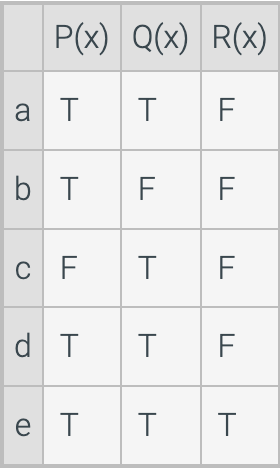
\includegraphics[width=0.2\textwidth]{screenshot1.png}
        \end{figure}
        \begin{enumerate}
            \item \[\exists x ((x=c) \rightarrow P(x))\]
            \item \[\exists x (Q(x) \land R(x))\]
            \item \[Q(a) \land P(d)\]
            \item \[\forall x ((x \neq b) \rightarrow Q(x))\]
            \item \[\forall x (P(x) \lor R(x))\]
            \item \[\forall x (R(x) \rightarrow P(x))\]
            \item \[\exists x (Q(x) \lor R(x))\]
        \end{enumerate}
        \textbf{Solution}
        \begin{enumerate}
            \item true
            \item true
            \item true
            \item true
            \item false
            \item true
            \item true
        \end{enumerate}
        \item Exercise 1.9.2, sections b - i\\
        \\The tables below show the values of predicates P(x, y), Q(x, y), and S(x, y) for every possible combination of values of the variables x and y. The row number indicates the value for x and the column number indicates the value for y. The domain for x and y is {1, 2, 3}.
        \begin{figure}[H]
            \centering
            \includegraphics*[width=0.5\textwidth]{screenshot2.png}
        \end{figure}
        Indicate whether each of the quantified statements is true or false.\\
        \begin{enumerate}
            \item \[\exists x\;\forall y \;Q(x, y)\]
            \item \[\exists y \;\forall x \;P(x, y)\]
            \item \[\exists x \;\exists y \;S(x, y)\]
            \item \[\forall x \;\exists y \;Q(x, y)\]
            \item \[\forall x \;\exists y \;P(x, y)\]
            \item \[\forall x \;\forall y \;P(x, y)\]
            \item \[\exists x \;\exists y \;Q(x, y)\]
            \item \[\forall x \;\forall y \;\neg S(x, y)\]
        \end{enumerate}
        \textbf{Solution}
        \begin{enumerate}
            \item true
            \item false
            \item false
            \item false
            \item true
            \item false
            \item true
            \item true
        \end{enumerate}
    \end{enumerate}

\end{homeworkProblem}

\pagebreak

\begin{homeworkProblem}
    Solve the following questions from the Discrete Math zyBook:
    \begin{enumerate}
        \item Exercise 1.10.4, sections c - g\\
        \\
        Translate each of the following English statements into logical expressions. The domain is the set of all real numbers.\\
        \begin{enumerate}
            \item There are two numbers whose sum is equal to their product.
            \item The ratio of every two positive numbers is also positive.
            \item The reciprocal of every positive number less than one is greater than one.
            \item There is no smallest number.
            \item Every number other than 0 has a multiplicative inverse.
            \item Every number other than 0 has a unique multiplicative inverse.
        \end{enumerate}

        \textbf{Solution}
        \begin{enumerate}
            \item \[\exists x \;\exists y \;(x+y=xy)\]
            \item \[\forall x \;\forall y \;(\frac{x}{y}>0)\]
            \item \[\forall x \;((x<1) \rightarrow (\frac{1}{x}>1))\]
            \item \[\forall x \;\exists y \;(y<x)\]
            \item \[\forall x \;\exists y ((x \neq 0) \rightarrow (xy = 1))\]
            \item \[\forall x \;\exists y \;\forall z \;(x \neq 0 \rightarrow xy = 1 \land z \neq y \rightarrow xz \neq 1)\]\\
        \end{enumerate}
        \item Exercise 1.10.7, sections c - f\\
        \\
        The domain is a group working on a project at a company. One of the members of the group is named Sam. Define the following predicates.\\
        \\
        P(x, y): x knows y's phone number. (A person may or may not know their own phone number.)\\
        D(x): x missed the deadline.\\
        N(x): x is a new employee.\\
        \\
        Give a logical expression for each of the following sentences.\\
        \begin{enumerate}
            \item There is at least one new employee who missed the deadline.
            \item Sam knows the phone number of everyone who missed the deadline.
            \item There is a new employee who knows everyone's phone number.
            \item Exactly one new employee missed the deadline.
        \end{enumerate}

        \textbf{Solution}
        \begin{enumerate}
            \item \[\exists x\;D(x)\]
            \item \[\forall y \; (P(Sam, y) \rightarrow D(y))\]
            \item \[\exists x \;\forall y \;P(x, y)\]
            \item \[\exists x \;\forall y \;(D(x) \land N(x) \land (y \neq x) \land (N(y) \rightarrow \neg D(y)))\]\\
        \end{enumerate}
        \item Exercise 1.10.10, sections c – f\\
        \\
        The domain for the first input variable to predicate T is a set of students at a university. The domain for the second input variable to predicate T is the set of Math classes offered at that university. The predicate T(x, y) indicates that student x has taken class y. Sam is a student at the university and Math 101 is one of the courses offered at the university. Give a logical expression for each sentence.\\

        \begin{enumerate}
            \item Every student has taken at least one class other than Math 101.
            \item There is a student who has taken every math class other than Math 101.
            \item Everyone other than Sam has taken at least two different math classes.
            \item Sam has taken exactly two math classes.
        \end{enumerate}
        
        \textbf{Solution}
        \begin{enumerate}
            \item \[\forall x \;\exists y \;((y \neq Math 101) \rightarrow T(x, y))\]
            \item \[\exists x \;\forall y \;((y \neq Math 101) \rightarrow T(x, y))\]
            \item \[\forall x \;\exists y \;\exists z \;((x \neq Sam) \land T(x, y) \land (z \neq y) \rightarrow T(x, z))\]
            \item \[\exists x \;\exists y \;\forall z \;((x \neq y) \land T(Sam, x) \land T(Sam, y) \land (z \neq x \land z \neq y) \rightarrow \neg T(Sam, z))\]
        \end{enumerate}
    \end{enumerate}
\end{homeworkProblem}

\pagebreak

\begin{homeworkProblem}
    Solve the following questions from the Discrete Math zyBook:
    \begin{enumerate}
        \item Exercise 1.8.2, sections b – e\\
        \\
        In the following question, the domain is a set of male patients in a clinical study. Define the following predicates:\\
        \\
        P(x): x was given the placebo\\
        D(x): x was given the medication\\
        M(x): x had migraines\\
        \\
        Translate each statement into a logical expression. Then negate the expression by adding a negation operation to the beginning of the expression. Apply De Morgan's law until each negation operation applies directly to a predicate and then translate the logical expression back into English.\\
        \begin{enumerate}
            \item Every patient was given the medication or the placebo or both.
            \item There is a patient who took the medication and had migraines.
            \item Every patient who took the placebo had migraines. 
            \item There is a patient who had migraines and was given the placebo.
        \end{enumerate}

        \textbf{Solution}
        \begin{enumerate}
            \item 
            \begin{enumerate}{i.}
                \item \[\forall x \;(D(x) \lor P(x))\]
                \item Negation: \[\exists x \;\neg (D(x) \lor P(x))\]
                \item Applying De Morgan's Laws: \[\exists x \;(\neg D(x) \land \neg P(x))\]
                \item Translation: There is at least one patient that was not given the placebo and the medication.
            \end{enumerate}
            \item
            \begin{enumerate}{i.}
                \item \[\exists x \;(D(x) \land M(x))\]
                \item Negation: \[\forall x \;\neg (D(x) \land M(x))\]
                \item Applying De Morgan's Laws: \[\forall x \;(\neg D(x) \lor \neg M(x))\]
                \item Translation: Every patient was either not given medication or not had migraines
            \end{enumerate}
            \item
            \begin{enumerate}{i.}
                \item \[\forall x \;(P(x) \rightarrow M(x))\]
                \item Negation: \[\exists x \;\neg (\neg P(x) \lor M(x))\] 
                \item Applying De Morgan's Laws: \[\exists x \;(P(x) \land \neg M(x))\]
                \item Translation: There is at least one patient was given the placebo and not had migraines.
            \end{enumerate}
            \item 
            \begin{enumerate}{i.}
                \item \[\exists x \;(M(x) \land P(x))\]
                \item Negation: \[\forall x \;\neg (M(x) \land P(x))\]
                \item Applying De Morgan's Laws: \[\forall x \;(\neg M(x) \lor \neg P(x))\]
                \item Translation: Every patient either did not have migraines or was not given the placebo or both.
            \end{enumerate}
        \end{enumerate}
        \item Exercise 1.9.4, sections c - e\\
        \\
        Write the negation of each of the following logical expressions so that all negations immediately precede predicates. In some cases, it may be necessary to apply one or more laws of propositional logic.\\
        \begin{enumerate}
            \item \[\exists x \;\forall y \;(P(x, y) \rightarrow Q(x, y))\]
            \item \[\exists x \;\forall y \;(P(x, y) \leftrightarrow P(y, x))\]
            \item \[\exists x \;\exists y \;P(x, y) \land \forall x \;\forall y \;Q(x, y)\]
        \end{enumerate}

        \textbf{Solution}
        \begin{enumerate}
            \item \[\neg \exists x \;\forall y \;(P(x, y) \rightarrow Q(x, y))\]
            \[\iff \forall x \;\exists y \; \neg (P(x, y) \rightarrow Q(x, y))\] (De Morgan's Laws)
            \[\iff \forall x \;\exists y \; \neg (\neg P(x, y) \lor Q(x, y))\] (Conditional Identities)
            \[\iff \forall x \;\exists y \; (P(x, y) \land \neg Q(x, y))\] (De Morgan's Laws)\\
            \item \[\exists x \;\forall y \;(P(x, y) \leftrightarrow P(y, x))\]
            \[\iff \forall x \;\exists y \; \neg ((P(x, y) \rightarrow P(y, x)) \land (P(y, x) \rightarrow P(x, y)))\] (Conditional Identities)
            \[\iff \forall x \;\exists y \; \neg ((\neg P(x, y) \lor P(y,x)) \land (\neg P(y, x) \lor P(x, y)))\] (De Morgan's Laws)
            \[\iff \forall x \;\exists y \; (\neg (\neg P(x, y) \lor P(y, x)) \lor \neg (\neg P(y, x) \lor P(x, y)))\] (De Morgan's Laws)
            \[\iff \forall x \;\exists y \; ((P(x, y) \land \neg P(y, x)) \lor (P(y, x) \land \neg P(x, y)))\]\\
            \item \[\exists x \;\exists y \;P(x, y) \land \forall x \;\forall y \;Q(x, y)\]
            \[\iff \neg (\exists x \;\exists y \;P(x, y) \land \forall x \;\forall y \;Q(x, y))\]
            \[\iff \forall x \; \forall y \; \neg P(x, y) \lor \exists x \; \exists y \; \neg Q(x, y)\] (De Morgan's Laws)
        \end{enumerate}
    \end{enumerate}
\end{homeworkProblem}

\end{document}